\documentclass{beamer}
\usepackage[utf8]{inputenc}
\usepackage{fancyvrb}
\usepackage{xcolor}
%\usetheme{Warsaw}
%\usetheme{JuanLesPins}
%\usetheme{Copenhagen}
\usetheme{Antibes}


\title{Sécurité: Virus}
\author{Mohamed El-Had Mellany - Mouagni Anas}
\institute{UM2}
\date{6 Décembre 2012}

\AtBeginSection[]
{
	\begin{frame}
		\frametitle{Sommaire}
		\tableofcontents[currentsection, hideothersubsections]
	\end{frame}
}

\begin{document}

\begin{frame}
	\titlepage
\end{frame}


\section{Introduction}
\begin{frame}
	\frametitle{Introduction}
	Un logiciel malveillant est un programme développé dans le but de nuire à un système informatique.
\end{frame}

\section{Qu'est-ce qu'un virus ?}
\subsection{Définition}
\begin{frame}
	\frametitle{Définition}
		Un virus est un programme susceptible de s'introduire dans un système, de s'y exécuter et qui tend à se propager de machines en machines par un mécanisme de réplication.
\end{frame}

\subsection{Origine}
\begin{frame}
\begin{itemize}
	\frametitle{Origine}
	\item 1949: Jhon Von Neumann présente les fondements théorique des logiciels autocopié.\newline
	\item 1960: Un groupe d'ingénieur des laboratoire Bell met au point un jeu informatique du nom de Core War.\newline
	\item 1983: Le premier virus fut créé par Fred Cohen.\newline
	\end{itemize}
\end{frame}
\begin{frame}
\begin{itemize}
\frametitle{Origine}
	\item Dans les années 80, les virus visent un ensemble de systèmes d'exploitation de réseaux.\newline
	\item Dans les années 90, ils servent surtout à dérober des informations confidentielles.\newline
	\item Les années 2000, ils utilisent les failles de Windows.
	\end{itemize}
\end{frame}
\begin{frame}
\frametitle{Systèmes d'exploitation les plus utilisés}
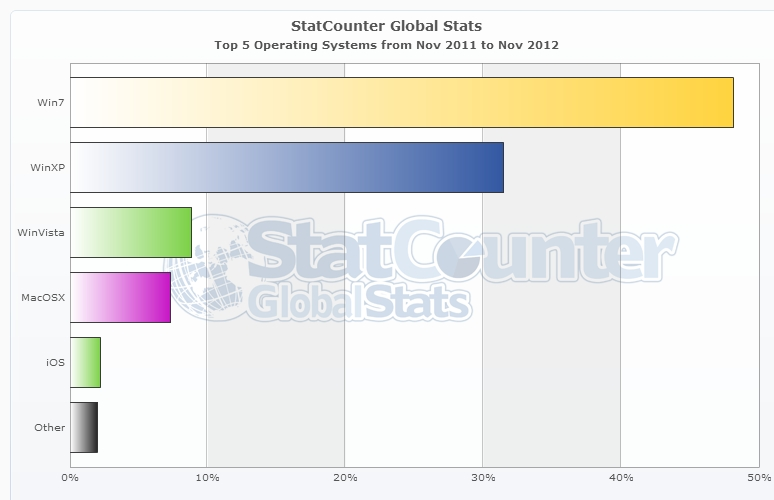
\includegraphics[scale=0.325]{graph1.jpg}
\end{frame}


\subsection{Les vecteurs de contamination}
\begin{frame}
\frametitle{Comment attrape-t-on un virus ?}
Un virus ne s'installe pas seul, il lui faut toujours un moyen pour arriver sur la machine et s’installer, on parle de vecteurs.
\end{frame}
\begin{frame}
\begin{itemize}
	\frametitle{Quels sont les vecteurs possibles ?}
	\item Le réseau (télèchargement http, pièce jointe dans un mail...)
	\pause\item Les périphériques (Disque Dur, clef USB)
	\pause\item Autres supports (DVD, CD, BlueRay)
\end{itemize}
\end{frame}

\subsection{Comment se reproduisent-ils ?}
\begin{frame}
	\frametitle{Comment se reproduisent-ils ?}
	Les virus se reproduisent en infectant un hôte: ajout d'un comportement malveillant à un programme existant.\newline
\end{frame}
\begin{frame}
\frametitle{Comment se reproduisent-ils ?}
Infection par écrasement et par recouvrement de code.
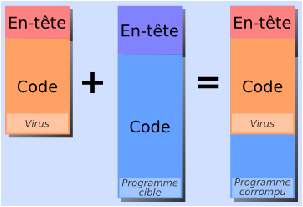
\includegraphics[scale=0.325]{graph2.png}
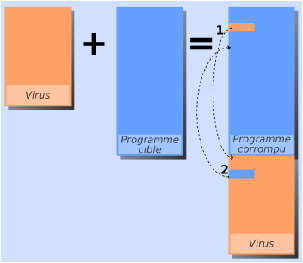
\includegraphics[scale=0.325]{graph3.png}
\end{frame}

\section{Les différentes familles}
\subsection{Familles}
\begin{frame}
	\frametitle{Familles}
	\begin{enumerate}
		\item virus de boot
		\pause\item virus polymorphique
		\pause\item virus furtif
		\pause\item virus chiffré
		\pause\item virus lié à l'horloge système
		\pause\item bombe logique
	\end{enumerate}
\end{frame}
\subsection{Le plus dangereux}
\begin{frame}
	\frametitle{Le plus dangereux}
	Tchernobyl (CIH), de 1998 à 2002 a fait environ 80 millions de dollars de dégâts.
\end{frame}



\section{Comment lutter ?}
\subsection{Antivirus}
\begin{frame}
	\begin{itemize}
	\frametitle{Antivirus ?}
		\item Qu'est ce qu'un antivirus ?
	\end{itemize}
\end{frame}
\begin{frame}
	\begin{itemize}
		\frametitle{Les techniques de détections}
		\item Signature
		\item Contrôleur d'intégrité
		\item Analyse spectrale
		\item Comportement
	\end{itemize}
	\end{frame}

\section{Quelles sont les failles exploitées ?}
\begin{frame}
	\frametitle{Quelles sont les failles exploitées}
	%graphique
	Graphique des vulnérabilités exploitées par les codes malveillants
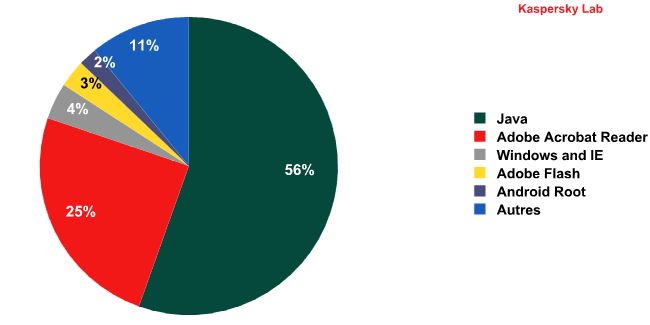
\includegraphics[scale=0.325]{graph4.png}
\end{frame}


\section{Les virus dans le monde}
\subsection{Les pays hébergeurs de programmes malveillants}
\begin{frame}
	\frametitle{Les pays hébergeurs de programmes malveillants}
	%graph
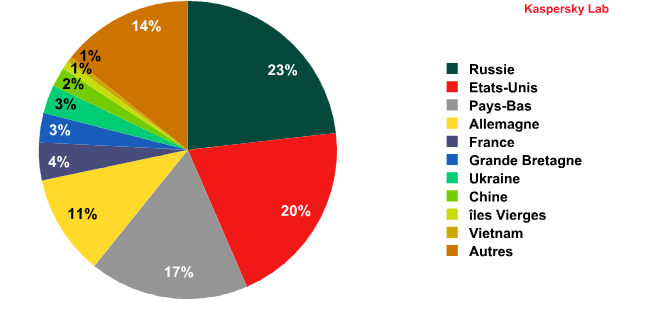
\includegraphics[scale=0.325]{graph5.png}
\end{frame}

\subsection{Pays dont les internautes ont été les plus exposés}
\begin{frame}
	\frametitle{Pays dont les internautes ont été les plus exposés}
	%graph
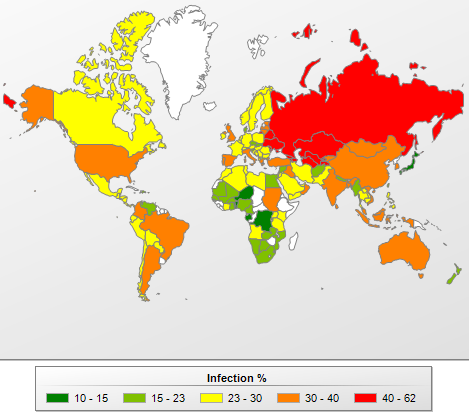
\includegraphics[scale=0.325]{graph6.png}
\end{frame}



\section{Conclusion}
\begin{frame}
	\frametitle{Conclusion}
	Les virus ont été créés dans un but expérimental, puis l’idée a été reprise pour en faire des programmes malveillants.\newline
	Le principal vecteur se trouve généralement entre la chaise et le clavier.\newline
	De nos jours, les virus sont devenus des armes employées dans des cyber-guerres menées par certains états.\newline
	Ne pas se soucier de la sécurité de ses machines fait potentiellement de l'utilisateur un participant passif de la cyber-criminalité.
\end{frame}
\begin{frame}
\frametitle{Sources}
Les réseaux - G. Pujolle - Edition2011\newline
http://vaccin.sourceforge.net/docs/definition2.html\newline
http://fr.wikipedia.org/\newline
http://www.infos-du-net.com/actualite/dossiers/112-2-histoire-virus.html\newline
http://www.commentcamarche.net/news/5856869-le-systeme-d-exploitation-windows-7-devient-le-plus-utilise-dans-le-monde\newline
http://vaccin.sourceforge.net/docs/definition2.html\newline
http://securite.topnet.tn/\newline
http://www.viruslist.com/fr/viruses/analysis\newline


\end{frame}

\end{document}
